% !TEX encoding = UTF-8 Unicode
\chapter{Umsetzung}
In diesem Kapitel wird beschrieben, wie Esper installiert werden kann. Die in der Implementierung entwickelte Java-Anwendung, verwendet Esper im Kontext des Szenarios (siehe Kapitel \ref{Szenario}) dieser Arbeit.
\section{Installation}
Für die Installation von Esper wird in dieser Ausarbeitung des Build-Tool \textbf{Apache Maven} verwendet. 
Dieses ermöglicht das automatisierte Herunterladen der Esper-Engine. Hierzu wird eine Konfigurationsdatei für Maven benötigt, die sogenannte \textbf{pom.xml}. Nachfolgend wird diese für das Szenario dargestellt:

\begin{lstlisting}[caption={Maven-Konfiguration}\label{lst:mavenKonfiguration},captionpos=t,language=XML]

<?xml version="1.0" encoding="UTF-8"?>
    <project xmlns="http://maven.apache.org/POM/4.0.0"
     xmlns:xsi="http://www.w3.org/2001/XMLSchema-instance"
     xsi:schemaLocation="http://maven.apache.org/POM/4.0.0
     http://maven.apache.org/xsd/maven-4.0.0.xsd">
		
     <modelVersion>4.0.0</modelVersion>

     <groupId>de.htwg.da</groupId>
     <artifactId>esper-sample</artifactId>
     <version>1.0-SNAPSHOT</version>

     <dependencies>
         <dependency>
             <groupId>com.espertech</groupId>
             <artifactId>esper</artifactId>
             <version>7.1.0</version>
         </dependency>
     </dependencies>
</project>
\end{lstlisting}

Wichtig ist hierbei das XML-Element \textbf{<dependencies>} welche die Abhängigkeiten enthält. Diese werden automatisch heruntergeladen, sobald Maven ausgeführt wird. In der Beispiel-Konfiguration gibt es nur eine Abhängigkeit, die für Esper.

Nach dem Download kann die Esper-Engine direkt bei der Entwicklung einer Java-Anwendung verwendet werden. Für andere Sprachen, sind unter Umständen Build-Tools zu verwenden, welche hier nicht beschrieben werden.


\section{Implementierung}
\begin{figure}[ht]
	\centering
	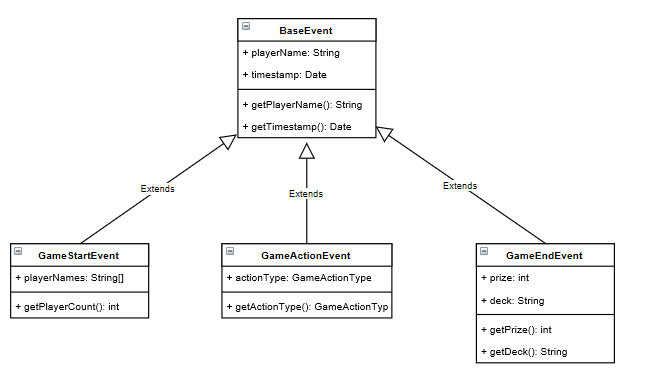
\includegraphics[width=\textwidth,height=\textheight,keepaspectratio]{images/Events.png}
	\caption{Event Klassen des Szenarios}
	\label{EventKlassen}
\end{figure}
Um das Szenario abzubilden werden verschiedene Event-Klassen benötigt. Mit diesem Begriff sind Klassen gemeint, die ein Event darstellen.
Als gemeinsame Basis dient die Event-Klasse \textbf{BaseEvent} (Siehe Abbildung \ref{EventKlassen}). Dieses Event beinhaltet den Spieler-Namen und einen Zeitstempel. Diese beiden Felder werden in allen Events benötigt.

Die Event-Klassen \textbf{GameStartEvent} und \textbf{GameEndEvent} bilden den Start und das Ende einer Poker-Partie ab. Zu Beginn (GameStartEvent) werden alle Spiel-Teilnehmer benötigt, gegen Ende (GameEndEvent) das Preisgeld und Kartendeck, welches gewonnen hat. Da beide Events von \textbf{BaseEvent} erben, besitzen sie automatisch auch einen Zeitstempel und den zugeordneten Spieler. Beim Spielstart ist der zugeordnete Spieler-Name, der Name des ersten Spielers.

Im Laufe der Partie werden verschiedene Aktionen der Spieler durchgeführt. Diese sind durch die Event-Klasse \textbf{GameActionEvent} abgebildet. Das Event beinhaltet ein Feld für die Aktionsart (z.B. "rise", wenn ein Spieler erhöht hat).